\documentclass[12pt]{article}
\usepackage[utf8x]{inputenc}
\usepackage{amsmath}
\usepackage{graphicx}
\usepackage{float}
\usepackage{array}
\usepackage{dsfont}
\usepackage{amsfonts}
\usepackage{lipsum}
\usepackage{enumitem}
\usepackage{epstopdf}
\usepackage[T1]{fontenc}
\usepackage[colorinlistoftodos]{todonotes}
\usepackage[left=2cm,right= 2cm,top=3cm,bottom=2.5cm,a4paper]{geometry}
\usepackage{listings}
\usepackage{xcolor}
\usepackage{multicol}
\usepackage{fancyhdr}
\usepackage{caption}
\usepackage{cite}
\usepackage{siunitx}
\setlength{\columnsep}{1cm}
\setlength{\parindent}{0pt}
\newcommand{\deriv}{\mathrm{d}}
\usepackage{color}  
\usepackage{hyperref}
\usepackage{cleveref}
\hypersetup{
    colorlinks=true, 
    linktoc=all,    
    linkcolor=black,
    citecolor=black,
}
\lstset{
    language=R,
    basicstyle=\scriptsize\ttfamily,
    commentstyle=\ttfamily\color{red},
    numbers=left,
    numberstyle=\ttfamily\color{blue}\footnotesize,
    stepnumber=1,
    numbersep=5pt,
    backgroundcolor=\color{white},
    showspaces=false,
    showstringspaces=false,
    showtabs=false,
    frame=single,
    tabsize=2,
    captionpos=b,
    breaklines=true,
    breakatwhitespace=false,
    title=\lstname,
    escapeinside={},
    keywordstyle={},
    morekeywords={}
}

\pagestyle{fancy}
\fancyhf{}
\rhead{PH370 Physics Labs}
\lhead{LLR.3 - Deduction of a Law}
\rfoot{-\thepage\centering-}

\begin{document}
\begin{titlepage}

\newgeometry{left=1.5in,right=1.5in,top=2.5in,bottom=2.5in}
\newcommand{\HRule}{\rule{\linewidth}{0.5mm}}

\begin{centering} 
 
%------------------------------------------------------------------------
%	HEADING SECTIONS
%------------------------------------------------------------------------


\includegraphics[scale=0.4]{Media/Uni_of_Kent_Logo.png}\\[1cm]

%------------------------------------------------------------------------
%	TITLE SECTION
%------------------------------------------------------------------------

\HRule \\[0.4cm]
\textsc{\large Astronomy, Space Science and Astrophysics}\\[0.4cm]
{\huge \bfseries Deduction of a Law}\\[0.4cm]
\HRule \\[1.0cm]

%------------------------------------------------------------------------
%	DATE SECTION
%------------------------------------------------------------------------

\textsc{\Large Stage 1 - PH370 Physics Labs}\\[0.5cm] 
{\large Monday 5th/12th March 2018}\\[1.0cm]

%------------------------------------------------------------------------
%	AUTHOR SECTION
%------------------------------------------------------------------------

\begin{minipage}{0.625\textwidth}
\centering

\emph{\large Report Author:} \large Lukasz R Tomaszewski \\ [0.2cm]
\emph{\large Lab Partner:} \large Holly L Stoke-Geddes \\

\end{minipage}\\[2cm]

\vfill
\end{centering} 
\end{titlepage}

%------------------------------------------------------------------------
%------------------------------------------------------------------------
%	CONTENTS  
%------------------------------------------------------------------------
%------------------------------------------------------------------------

\newpage
\begin{titlepage}
\begin{tableofcontents}

\end{tableofcontents}
\end{titlepage}

%-----------------------------------------------------------------------
%-----------------------------------------------------------------------
%	ABSTRACT
%-----------------------------------------------------------------------
%-----------------------------------------------------------------------

\section{Abstract}
\label{Abstract Section}

Within this experiment, using \cite{LLR.3-2018} as a guide, will prove if a materials physical property has any change on its period of oscillation, it will be found that in small changes of its specific physical property, no change is seen in terms of its period of oscillation. Only in larger value differences will the period of oscillation see significant change. 

%-----------------------------------------------------------------------
%-----------------------------------------------------------------------
%	INTRODUCTION
%-----------------------------------------------------------------------
%-----------------------------------------------------------------------

\section{Introduction}
\label{Introduction Section}

This is quite a short scripted experiment, the purpose is to find the relationship between the period of a mechanical oscillator via physical properties e.g. mass, volume, area, thickness, density and side length. This will be done first empirically and then theoretically, when completed the moment of inertia of a rectangular parallelepiped about axis through centre perpendicular to its face, this will be then used to calculate the acceleration due to gravity.

%-----------------------------------------------------------------------
%-----------------------------------------------------------------------
%	AIMS & EQUIPMENT
%-----------------------------------------------------------------------
%-----------------------------------------------------------------------

\section{Aims \& Equipment}
\label{AimsEquipmentSection}

%-----------------------------------------------------------------------
%	APPARTUS
%-----------------------------------------------------------------------

\subsection{Apparatus}
\label{Apparatus SubSection}

\begin{multicols}{3}
\begin{itemize}
    \item{Electronic scales}
    \item{Bosshead}
    \item{30cm steel rule}
    \item{Graph paper}
    \item{Suspension bar}
    \item{Stop clock}
    \item{Retort stand}
    \item{Metre rule}
    \item{Various sized metal/ plastic squares}
    \item{x4 Metal square (20cm x 20cm)}
\end{itemize}
\end{multicols}

%-----------------------------------------------------------------------
%	DATA COLLECTED
%-----------------------------------------------------------------------

\subsection{Data Collected}
\label{Data Collected SubSection}

\begin{multicols}{3}
\begin{itemize}
    \item{Mass of squares}
    \item{Area of squares}
    \item{Density of squares}
    \item{Thickness of squares}
    \item{Volume of squares}
    \item{Length of sides of squares}
    \item{The period of oscillation}
    \item{Acceleration due to gravity}
\end{itemize}
\end{multicols}

%-----------------------------------------------------------------------
%	RISK ASSESSMENT
%-----------------------------------------------------------------------

\subsection{Risk Assessment}
\label{Risk Assessment SubSection}

In this experiment, there are two potential hazards that could occur. The first involves swinging metal plates, the second is equipment falling off the desk. Both of these hazards have the potential to cause bruising/ injury to feet and the lower body. \\

The above hazards can be controlled by moving the equipment away from the edges of the desk and keeping them in the middle of the desk, the retort stand will be secured to the desk via a G-clamp.

%-----------------------------------------------------------------------
%-----------------------------------------------------------------------
%	EXPERIMENTAL PROCEDURE
%-----------------------------------------------------------------------
%-----------------------------------------------------------------------

\section{Experimental Procedure}
\label{Experimental Procedure Section}

The experiment started by selected squares with one similar physical property e.g. area, thickness, density and side length. This fixed variable was the same for five selected squares, five square for each one fixed physical property, this allows for a fair analysis when comparing how the fixed physical property affects the period of oscillation. When selecting a fixed physical property, each of the five squares are measured for different physical properties e.g. mass, volume, area, thickness, density and side length. The measurement of the varied physical property each square contains has the potential to alter the individual squares period of oscillation. \\

As the squares are of small measurement and the angle of attack is large, there is a lot of potential human error when timing the period of oscillation, thus to deter the amount of human error that affects the recording of the period of oscillation, the squares will complete 20 oscillations fully timed, then will divide the overall time by 20 to get one period of oscillation for each square. Then the period of oscillations for each square will be plotted against their own chosen physical property. \\

%-----------------------------------------------------------------------
%-----------------------------------------------------------------------
%	RESULT & DISSCUSSION
%-----------------------------------------------------------------------
%-----------------------------------------------------------------------

\section{Results \& Discussion}
\label{Results Discussion Section}

%-----------------------------------------------------------------------
%	Task 3.1 - Moment of Inertia
%-----------------------------------------------------------------------

\subsection{Task 3.1 - Moment of Inertia}
\label{Task 3.1 - Moment of Inertia SubSection}

Moment of Inertia for a rectangle through its centre of mass; \\

\begin{equation} \label{Moment of Inertia for a rectangle}
{I_{cm} = M \times (a^2 + b^2)}
\end{equation}

\begin{equation*}
\begin{split}
&\text{Where;} \\
&I_{cm} \Rightarrow \text{Moment of Inertia at centre of mass} \\
&a+b \Rightarrow \text{Height \& length of rectangle} \\
&M \Rightarrow \text{Mass} \\
\end{split}
\end{equation*} \\

Parallel Axis Theorem ; \\

\begin{equation} \label{Parallel Axis Theorem}
{I = I_{cm} + (M \times h^2)}
\end{equation}

\begin{equation*}
\begin{split}
&\text{Where;} \\
&I_{cm} \Rightarrow \text{Moment of Inertia at centre of mass} \\
&h \Rightarrow \text{Distance between centre of mass and pivot} \\
&M \Rightarrow \text{Mass} \\
\end{split}
\end{equation*} \\

Therefore;

\begin{equation} \label{Final}
{I = (M \times (a^2 + b^2)) + (M \times h^2)}
\end{equation}

\begin{equation*}
\begin{split}
&\text{Where;} \\
&h \Rightarrow \text{Distance between centre of mass and pivot} \\
&a+b \Rightarrow \text{Height \& length of rectangle} \\
&M \Rightarrow \text{Mass} \\
\end{split}
\end{equation*} \\

%-----------------------------------------------------------------------
%	Task 3.2 - Period of Oscillation
%-----------------------------------------------------------------------

\subsection{Task 3.2 - Period of Oscillation}
\label{Task 3.2 - Period of Oscillation}

\begin{multicols}{2}
\begin{table}[H]
\centering
\caption{Area vs Period}
\label{Area vs Period}
\begin{tabular}{lllllll}
Area (mm\textasciicircum 2) & Period (s) \\
22,201                      & 0.705                     \\
12,100                      & 0.622                     \\
3,136                       & 0.433                     \\
2,401                       & 0.422                     \\
4,900                       & 0.472                    
\end{tabular}
\end{table}

\begin{table}[H]
\centering
\caption{Density Vs Period}
\label{Density Vs Period}
\begin{tabular}{lllllll}
Density (g/mm\textasciicircum 3) & Period (s) \\
1.156x10\textasciicircum \{-3\}  & 0.716      \\
9.978x10\textasciicircum \{-4\}  & 0.708      \\
1.216x10\textasciicircum \{-3\}  & 0.702     
\end{tabular}
\end{table}

\begin{table}[H]
\centering
\caption{Thickness Vs Period}
\label{Thickness Vs Period}
\begin{tabular}{llllll}
Thickness (mm) & Period (s) \\
3.02           & 0.844      \\
5.01           & 0.819      \\
7.96           & 0.835      \\
10.06          & 0.832      \\
11.96          & 0.827     
\end{tabular}
\end{table}

\begin{table}[H]
\centering
\caption{Side Length Vs Period}
\label{Side Length Vs Period}
\begin{tabular}{lllllll}
Side Length (mm) & Period (s) \\
149              & 0.705                     \\
110              & 0.622                     \\
56               & 0.433                     \\
49               & 0.422                     \\
70               & 0.472                    
\end{tabular}
\end{table}
\end{multicols}

%-----------------------------------------------------------------------
%	Task 3.3 - Physical Properties Vs Period Graphs
%-----------------------------------------------------------------------

\pagebreak
\subsection{Task 3.3 - Physical Properties Vs Period Graphs}
\label{Task 3.3 - Physical Properties Vs Period Graphs}

\begin{table}[H]
\centering
\caption{Period Vs Area Results}
\label{Period Vs Area Results}
\begin{tabular}{lllllll}
Side Length (mm) & Thickness (mm) & Area (mm\textasciicircum 2) & Volume (mm\textasciicircum 3) & Mass (g) & Period (s) \\
149              & 4.89           & 22,201                      & 108,592.23                    & 134.12   & 0.705                     \\
110              & 4.86           & 12,100                      & 58,806                        & 41.20    & 0.622                     \\
56               & 4.88           & 3,136                       & 15,303.68                     & 23.84    & 0.433                     \\
49               & 4.76           & 2,401                       & 11,428.76                     & 16.68    & 0.422                     \\
70               & 4.78           & 4,900                       & 22,422                        & 31.78    & 0.472                    
\end{tabular}
\end{table}

\begin{table}[H]
\centering
\caption{Period Vs Density Results}
\label{Period Vs Density Results}
\begin{tabular}{lllllll}
Side Length (mm) & Thickness (mm) & Volume (mm\textasciicircum 3) & Density (g/mm\textasciicircum 3) & Mass (g) & Period (s) \\
149              & 4.98           & 110,560.98                    & 1.156x10\textasciicircum \{-3\}  & 127.85   & 0.716      \\
149              & 4.98           & 110,560.98                    & 9.978x10\textasciicircum \{-4\}  & 110.32   & 0.708      \\
149              & 4.98           & 110,560.98                    & 1.216x10\textasciicircum \{-3\}  & 134.46   & 0.702     
\end{tabular}
\end{table}

\begin{multicols}{2}

\begin{figure}[H]
\centering
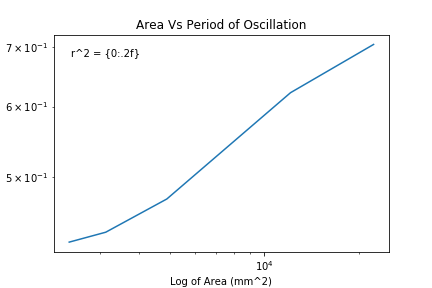
\includegraphics[scale=0.6]{Media/Area_Vs_Period.png}
\caption{Area Vs Period Graph.}
\label{Area Vs Period Graph}
\end{figure}

\begin{table}[H]
\centering
\caption{Area vs Period}
\label{Area vs Period}
\begin{tabular}{lllllll}
Log of Area (mm\textasciicircum 2) & Log of Period (s) \\
10.0078926                      & -0.3495575                     \\
9.40096073                      & -0.4748152                     \\
8.05070338                       & -0.8370176                     \\
7.7836406                       & -0.86275                     \\
8.49699048                       & -0.7507763                    
\end{tabular}
\end{table}

\begin{figure}[H]
\centering
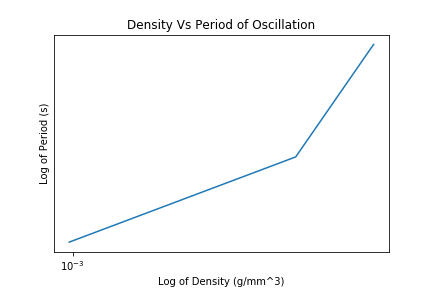
\includegraphics[scale=0.6]{Media/Density_Vs_Period.png}
\caption{Density Vs Period Graph.}
\label{Density Vs Period Graph}
\end{figure}

\begin{table}[H]
\centering
\caption{Density Vs Period}
\label{Density Vs Period}
\begin{tabular}{lllllll}
Log of Density (g/mm\textasciicircum 3) & Log of Period (s) \\
-6.7627895  & -0.3347737      \\
-6.9099577  & -0.3460176      \\
-6.7121885  & -0.3545344     
\end{tabular}
\end{table}

\end{multicols}

\pagebreak

\begin{table}[H]
\centering
\caption{Period Vs Thickness Results}
\label{Period Vs Thickness Results}
\begin{tabular}{llllll}
Side Length (mm) & Thickness (mm) & Area (mm\textasciicircum 2) & Volume (mm\textasciicircum 3) & Mass (g) & Period (s) \\
200              & 3.02           & 40200                       & 121,404                       & 122.67   & 0.844      \\
200              & 5.01           & 40200                       & 608,234.04                    & 196.43   & 0.819      \\
200              & 7.96           & 40200                       & 4,841,542.958                 & 315.67   & 0.835      \\
200              & 10.06          & 40200                       & 48,705,922.16                 & 395.85   & 0.832      \\
200              & 11.96          & 40200                       & 582,522,829.10                & 469.78   & 0.827     
\end{tabular}
\end{table} 

\begin{table}[H]
\centering
\caption{Period Vs Side Length Results}
\label{Period Vs Side Length Results}
\begin{tabular}{lllllll}
Side Length (mm) & Thickness (mm) & Area (mm\textasciicircum 2) & Volume (mm\textasciicircum 3) & Mass (g) & Period (s) \\
149              & 4.89           & 22,201                      & 108,592.23                    & 134.12   & 0.705                     \\
110              & 4.86           & 12,100                      & 58,806                        & 41.20    & 0.622                     \\
56               & 4.88           & 3,136                       & 15,303.68                     & 23.84    & 0.433                     \\
49               & 4.76           & 2,401                       & 11,428.76                     & 16.68    & 0.422                     \\
70               & 4.78           & 4,900                       & 22,422                        & 31.78    & 0.472                    
\end{tabular}
\end{table}

\begin{multicols}{2}

\begin{figure}[H]
\centering
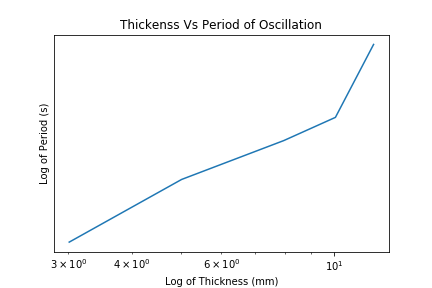
\includegraphics[scale=0.6]{Media/Thickness_Vs_Period.png}
\caption{Thickness Vs Period Graph.}
\label{Thickness Vs Period Graph}
\end{figure}

\begin{table}[H]
\centering
\caption{Thickness Vs Period}
\label{Thickness Vs Period}
\begin{tabular}{llllll}
Log of Thickness (mm) & Log of Period (s) \\
1.10194008           & -0.1696028      \\
1.61143592           & -0.2002819      \\
2.074429           & -0.1809225      \\
2.30856717          & -0.184524      \\
2.48156775          & -0.1905554     
\end{tabular}
\end{table}

\begin{figure}[H]
\centering
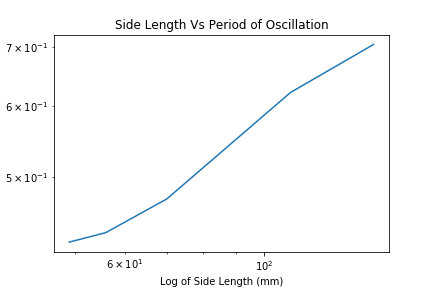
\includegraphics[scale=0.6]{Media/Side_Length_Vs_Period.png}
\caption{Side Length Vs Period Graph.}
\label{Side Length Vs Period Graph}
\end{figure}

\begin{table}[H]
\centering
\caption{Side Length Vs Period}
\label{Side Length Vs Period}
\begin{tabular}{lllllll}
Side Length (mm) & Period (s) \\
5.00394631              & -0.3502669                     \\
4.70048037              & -0.4748152                     \\
4.02535169               & -0.838173                     \\
3.8918203               & -0.86275                     \\
4.24849524               & -0.7507763                    
\end{tabular}
\end{table}

\end{multicols}

%-----------------------------------------------------------------------
%	THEORETICAL CONSIDERATIONS
%-----------------------------------------------------------------------

\pagebreak
\subsection{Theoretical Considerations}
\label{Theoretical Considerations SubSection}

Period of a Pendulum;

\begin{equation} \label{Period for Pendulum}
{T = 2\pi \times \sqrt{\dfrac{I}{Mgd}}}
\end{equation}

\begin{equation*}
\begin{split}
&\text{Where;} \\
&d \Rightarrow \text{Distance between centre of mass and pivot} \\
&g \Rightarrow \text{Gravitational Constant} \\
&I \Rightarrow \text{Moment of Inertia} \\
&M \Rightarrow \text{Mass} \\
\end{split}
\end{equation*} \\

Moment of Inertia for the Period for a Pendulum.

\begin{equation} \label{Moment of inertia for the period for a pendulum}
{T = 2\pi \times \sqrt{\dfrac{I}{Mgd}} \rightarrow 2\pi \times \sqrt{\dfrac{(a^2 + b^2)+h^2}{gd}}}
\end{equation} \\

%-----------------------------------------------------------------------
%	Task 4.1 - Theory Vs Empirical
%-----------------------------------------------------------------------

\subsection{Task 4.1 - Theory Vs Empirical}
\label{Task 4.1 Theory Vs Empirical SubSection}

Comparing both the theoretical formula in section \ref{Theoretical Considerations SubSection} against the empirical formulas received from the graphs, it can be seen that they are show no relationship.

%-----------------------------------------------------------------------
%	Task 4.2 - Acceleration due to Gravity
%-----------------------------------------------------------------------

\subsection{Task 4.2 - Acceleration due to Gravity}
\label{Task 4.2 - Acceleration due to Gravity SubSection}

\begin{equation}
{T = 2 \pi \times \sqrt{\dfrac{(a^2 + b^2)+h^2}{gd}}}
\end{equation} \\

\begin{equation} 
\left(\dfrac{T}{2\pi}\right)^2 = \dfrac{(a^2 + b^2)+h^2}{gd}
\end{equation} \\

\begin{equation}
\dfrac{(a^2 + b^2)+h^2}{\left(\dfrac{T}{2\pi}\right)^2} = gd
\end{equation} \\

\begin{equation}
g = \dfrac{(a^2 + b^2)+h^2}{d \left(\dfrac{T}{2\pi}\right)^2}
\end{equation} \\

%-----------------------------------------------------------------------
%	ANALYSIS
%-----------------------------------------------------------------------

\section{Analysis}
\label{Analysis Section}

Plotting the natural log of each physical property and its individual period of oscillation shows that their is not a clear relationship between these physical properties and the period of oscillation. By analyzing the graphs and tables, it shows little change when each physical property was larger or smaller, the period of oscillation remained the same with a small tolerance. The only physical property that changed the period of oscillation was Area, where even the second highest area produced a lower period whether this abnormality was due to human error or is practically proven is unclear but reviewing the results, human error seem to play a huge part within this experiment.  

%-----------------------------------------------------------------------
%	CONCLUSION
%-----------------------------------------------------------------------

\section{Conclusion}
\label{Conclusion Section}

In terms of the whole experiment, it was carried out in a fair standard. Within the mathematical side of the experiment, all measurements had fixed errors and no human error was at play but the physical measurement of the oscillation of each square was purely down to human error, where it was not truly fair and thus being inaccurate, there was delays in counting the oscillations by eye and starting/ stopping the stopwatch. All in all this experiment proved that physical properties do not have much effect in their periods of oscillation, only if the difference in each plates physical property was at a larger value may it be found that physical property changes the period of oscillation.

%------------------------------------------------------------------------
%	REFERENCES
%------------------------------------------------------------------------

\bibliographystyle{plain}
\bibliography{mybib}

%------------------------------------------------------------------------

\end{document}